% ============================================================
% DAETUM renderer regression fixture.
% A complete standalone LaTeX drawing document: everything that
% arrives at /api/render-tikz when a student pastes their own
% document into the Source tab.
%
% The renderer must process THIS document as given - its document
% class, its packages, its libraries, its document environment and
% its comments - without stripping the preamble or rewriting the
% drawing into other commands.
% ============================================================
\documentclass[tikz,border=5pt]{standalone}
\usepackage{tikz}
\usetikzlibrary{arrows.meta}
\usetikzlibrary{calc}

\begin{document}

\begin{tikzpicture}[x=1mm, y=1mm, scale=1]

  % ---- named points, the drawing's geometry of record ----
  \coordinate (A) at (0,0);
  \coordinate (B) at (60,0);
  \coordinate (C) at (30,35);

  % ---- the truss: two triangles sharing one side ----
  \draw[thick] (A) -- (B) -- (C) -- cycle;
  \draw[thick] (A) -- (C);

  % ---- a dashed reference line through the apex ----
  \draw[dashed, gray] (-10,0) -- (70,0);

  % ---- filled point markers at the nodes ----
  \fill (A) circle (1.2);
  \fill (B) circle (1.2);
  \fill (C) circle (1.2);

  % ---- mathematical node labels ----
  \node[below left]  at (A) {$A$};
  \node[below right] at (B) {$B$};
  \node[above]       at (C) {$C$};
  \node[below] at (30,-8) {$F_A = \tfrac{1}{2}wL$};

  % ---- a circular arc at the apex ----
  \draw (30,35) arc[start angle=180, end angle=300, radius=6];

  % ---- extension lines and a double-headed dimension arrow ----
  \draw[gray, thin] (0,40) -- (0,44);
  \draw[gray, thin] (60,40) -- (60,44);
  \draw[{Stealth[width=4mm]}-{Stealth[width=4mm]}] (0,42) -- (60,42)
    node[midway, above] {$L = 60\,\mathrm{mm}$};

  % ---- a load arrow on the apex ----
  \draw[-{Stealth[length=3mm]}] (30,55) -- (30,37)
    node[above] {$P$};

\end{tikzpicture}

\end{document}
